\documentclass{standalone}
\usepackage{tikz}
\usepackage{ctex,siunitx}
\setCJKmainfont{Noto Serif CJK SC}
\usepackage{tkz-euclide}
\usepackage{amsmath}
\usetikzlibrary{patterns, calc,3d}
\usetikzlibrary {decorations.pathmorphing,decorations.pathreplacing,decorations.shapes}
\tikzset{label style/.append style={font=\small}}
\begin{document}
\small
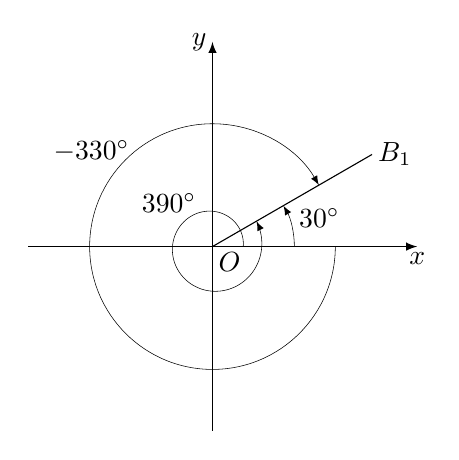
\begin{tikzpicture}[>=latex,scale=1.3,inner sep=2pt]
  \draw[->](-1.8,0)--(2,0)node[below]{$x$};
  \draw[->](0,-1.8)--(0,2)node[left]{$y$};
  \node at (0,0)[below right]{$O$};
  \draw(0,0)--(30:1.8)node[right]{$B_1$};
  \draw[very thin,->,samples=200,domain=0:390]plot(\x:{0.3+\x*0.0005});
  \draw[very thin,->](0.8,0)arc(0:30:0.8)node[pos=0.3,above right]{\ang{30}};
  \node at (135:0.6){\ang{390}};
  \draw[very thin,->](1.2,0)arc(0:-330:1.2)node[pos=0.7,left]{\ang{-330}};
\end{tikzpicture}
\end{document}